\documentclass[palatino, nochap]{apuntes}

\title{Diseño y Análisis de Algoritmos}
\author{Guillermo Julián Moreno}
\date{15/16 C1}

% Paquetes adicionales
\usepackage{minted}
\usepackage{fancysprefs}
\usepackage{tree}
\usepackage{tikz-qtree}
\usepackage{wrapfig}
\usepackage{booktabs}
\usepackage{colortbl}

% --------------------

\begin{document}
\pagestyle{plain}
\maketitle

\tableofcontents
\newpage

\section{Grafos}

Suponemos un cierto conocimiento básico sobre grafos. Denotaremos los grafo por $G = (V,E)$, con $V$ el conjunto de vértices o nodos y $E$ las aristas, donde $(u,v)$ con $u,v ∈ V$ es una arista que, en grafos dirigidos, implica dirección $u \to v$. Si el grafo es ponderado, los ejes tienen peso $w_{uv}$.

\subsection{Distancia mínima}

El problema se plantea fácilmente: dado un grafo $G$ y dos vértices $u$ y $v$, encontrar un camino mínimo $π = \set{u \equiv u_0, u_1, \dotsc, u_k \equiv v}$ de uno a otro.


\begin{listing}[hbtp]
\begin{minted}[frame=lines, fontsize=\scriptsize, tabsize=4]{python}
def dijkstra(G, from, costs, adjacent_nodes):
	n_nodes = len(G)
	visited = [False] * n_nodes
	path = [-1] * n_nodes
	distance = [infinity] * n_nodes
	queue = PriorityQueue()

	distance[from] = 0
	queue.put(from, priority = 0)

	while not q.empty():
		priority, node = queue.get()

		if not visited[node]:
			visited[node] = True

			for adj in adjacent_nodes[node]:
				if distance[adj] > distance[node] + costs[node, adj]:
					# Actualizamos el coste y el camino al nodo adyacente
					distance[adj] = distance[node] + costs[node, adj]
					path[adj] = node
					q.put(adj, priority = distance[adj])

	return path, distances
\end{minted}
\caption{Algoritmo de Dijkstra para encontrar los caminos mínimos a todos los nodos de un grafo $G$ dado un nodo incial.}
\label{lst:Dijkstra}
\end{listing}

Si el grafo no es ponderado, con una búsqueda en anchura (BFS) nos valdrá. Ahora bien, la cosa se complica en grafos ponderados. Para ello necesitaremos el \concept{Algoritmo\IS de Dijkstra} (\fref{lst:Dijkstra}), que usa una BFS con cola de prioridad. La prioridad de cada nodo es su distancia al nodo origen: cuanta menor es esa distancia, antes lo visitamos.

El coste de Dijkstra es $O(\abs{V} + \abs{E} \log \abs{V})$. Como explicación rápida, tenemos como mucho $\abs{E}$ aristas a meter en la cola de prioridad, que tendrá coste de inserción y extracción $O(\log \abs{E})$. Tenemos que recorrer todas las aristas, así que tendremos en total unas $O(\abs{E} \log \abs{E})$ operaciones. Como $\abs{E} = O(\abs{V}^2)$, lo que nos queda asintóticamente es $O(\abs{V} + \abs{E}\log \abs{V})$.

Cuando lo que queremos es buscar los caminos mínimos entre todos los pares de nodos, podemos usar un algoritmo algo mejor, especialmente para grafos densos donde el coste de Dijkstra iterado se va a $O(\abs{V}^3 \log \abs{V})$. Lo que usaremos en este caso será el \concept{Algoritmo\IS de Floyd-Warshall} (\fref{lst:FloydWarshall}), que tiene coste $O(\abs{V}^3)$.

\begin{listing}[hbtp]
\begin{minted}[frame=lines, fontsize=\scriptsize, tabsize=4]{python}

def floydWarshall(G):
	n_nodes = len(G)
	min_distances = G # Suponemos G dado como matriz.

	for k in range(node_count):
		for i in range(node_count):
			for j in range(node_count):
				if min_distances[i][j] > min_distances[i][k] + min_distances[k][j]:
					min_distances[i][j] = min_distances[i][k] + min_distances[k][j]

	return min_distances
\end{minted}
\caption{Algoritmo de Floyd-Warshall para encontrar todos los caminos mínimos entre los nodos de un grafo.}
\label{lst:FloydWarshall}
\end{listing}

\subsection{Árboles abarcadores}

La idea de un árbol abarcador es quedarnos con sólo un subconjunto $E_T ⊆ E$ de las aristas de un grafo, de tal forma que tengamos un árbol con todos los nodos del grafo original. BFS y DFS nos permiten generar estos árboles abarcadores, aunque querremos algo más sofisticado para sacar árboles con propiedades más específicas.

Por ejemplo, buscaremos árboles abarcadores mínimos, esto es, árboles $T = (V, E_T)$ tales que, para cualquier otro árbol abarcador $T' = (V, E_{T'})$, la suma de costes de las aristas $E_T$ sea menor que la de los costes de $E_{T'}$.

Un algoritmo para encontrar un árbol abarcador mínimo es el \concept{Algoritmo\IS de Prim} (\fref{lst:Prim}), que en el fondo no es más que una modificación ligera de Dijkstra en el que en lugar de mantener la tabla de distancias mantenemos una tabla de costes para cada arista del árbol. El coste de Prim es el mismo que el de Dijkstra, $O(\abs{E} \log \abs{V})$.


\begin{listing}[hbtp]
\begin{minted}[frame=lines, fontsize=\scriptsize, tabsize=4]{python}
def dijkstra(G, from, costs, adjacent_nodes):
	n_nodes = len(G)
	visited = [False] * n_nodes
	path = [-1] * n_nodes
	tree_costs = [infinity] * n_nodes
	queue = PriorityQueue()

	tree_costs[from] = 0
	queue.put(from, priority = 0)

	while not q.empty():
		priority, node = queue.get()

		if not visited[node]:
			visited[node] = True

			for adj in adjacent_nodes[node]:
				if tree_costs[adj] > costs[node, adj]
					# Actualizamos el coste y el camino al nodo adyacente
					tree_costs[adj] = costs[node, adj]
					path[adj] = node
					q.put(adj, priority = tree_costs[adj])

	return path, tree_costs
\end{minted}
\caption{Algoritmo de Prim para encontrar un árbol abarcador mínimo. El árbol se reconstruye recorriendo el array \texttt{path}: el nodo padre de $u$ es \texttt{path[u]} y la arista que los conecta tiene coste \texttt{tree\_costs[u]}.}
\label{lst:Prim}
\end{listing}

El otro algoritmo posible es el \concept{Algoritmo\IS de Kruskal}, probablemente más intuitivo. Se crea un bosque, al que por cada nodo se añade un árbol que consta únicamente de ese nodo. Después, se itera por cada rama, empezando por las de menor peso. Cada rama conecta dos nodos: si podemos (esto es, la rama no genera ciclos o, equivalentemente, los nodos están en árboles distintos), construimos un nuevo árbol uniendo los árboles en los que está cada nodo con la rama que consideramos. Al final nos quedará un único árbol (si no, es que el grafo no era conexo).

Para implementar el algoritmo (no vamos a poner el pseudocódigo) creamos un tipo abstracto de datos que representa la partición del conjunto de vértices $V$ y que nos permita realizar uniones de conjuntos.

Lo bueno es que un conjunto se puede representar por un árbol. A cada conjunto se le asigna un representante $u$, que consideraremos la raíz del árbol. Cada vértice del árbol es un elemento de ese conjunto. Unir dos árboles representados por elementos $u$ e $u$ será tan sencillo como hacer que $u$ sea un nodo hijo de $u$.

Así, podremos representar la partición por una matriz \texttt{p}, donde \texttt{p[u]} es el nodo padre de $u$ o, si $u$ es nodo raíz, valdrá $-1$. Luego todo esto se puede hacer más eficiente para que el coste de las uniones y de la búsqueda de un representante sea menor.

El algoritmo de Kruskal tiene coste $O(\abs{E} \log \abs{V})$ por las operaciones con la cola de prioridad.

\subsubsection{Invariantes de bucle}

Tanto Prim como Kruskal tienen una cosa en común: hay una condición que siempre se cumple tras cada iteración, que es que las aristas seleccionadas forman parte de un árbol abarcador mínimo. Esta condición se llama una \concept{Invariante\IS de bucle} y dan una idea de la corrección de algoritmos iterativos.

\subsection{Conexión en grafos}

\begin{wrapfigure}{r}{0.35\textwidth}
\centering
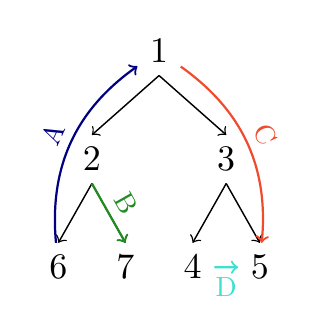
\begin{tikzpicture}[scale=1.3]
\tikzset{sibling distance=7pt}
\tikzset{edge from parent/.append style={->}}
\Tree [.\node(1) {1};
	[.\node(2) {2};
		[.\node (6) {6}; ]
		[.\node (7) {7}; ] ]
	[.3
		[.\node(4) {4}; ]
		[.\node(5) {5}; ] ]
]

\draw[NavyBlue, thick, ->] (6) to[bend left] node[midway, sloped, above] {A} (1);
\draw[ForestGreen, thick, ->] (2.south) to node[midway, sloped, above] {B} (7.north);
\draw[RedOrange, thick, ->] (1) to[bend left] node[midway, sloped, above] {C} (5);
\draw[Turquoise, thick, ->] (4) to node[midway, sloped, below] {D} (5);
\end{tikzpicture}
\caption{DFS induce una clasificación de las aristas de un grafo según cómo queden en el árbol.}
\label{fig:ArbolDFS}
\end{wrapfigure}

Para estudiar la conexión en grafos, se utilizan algoritmos derivados de la búsqueda en profundidad o DFS. Una de las primeras cosas que podemos ver es que las aristas $(u,v)$ se pueden clasificar según cómo queden en el árbol que genera DFS (\fref{fig:ArbolDFS}):

\begin{itemize}
\item \concept{Arista\IS árbol}: Aristas tipo B, donde $v$ es nodo hijo de $u$.
\item \concept{Arista\IS ascendentes}: Aristas tipo A, donde podemos llegar de $v$ a $u$ subiendo por el árbol.
\item \concept{Arista\IS descendentes}: Aristas tipo C, donde podemos llegar de $v$ a $u$ bajando por el árbol.
\item \concept{Arista\IS cruzada}: Aristas tipo D, básicamente cualquier otra que no quepa en la anterior clasificación.
\end{itemize}

En grafos no dirigidos, las aristas ascendentes y descendentes son iguales. Además, en ese caso tampoco hay aristas cruzadas (si queremos ir a un nodo que ya esté en el grafo, lo hemos visitado y por lo tanto DFS no pasará por ahí). La idea de esto viene de un teorema\footnote{Que por lo obvio que es no debería llamarse teorema ni de lejos.}, llamado \concept{Teorema\IS del paréntesis}. Si llevamos un conteo $c$ de cuántos nodos hemos visitado, y llamamos $d_u$ y $f_u$ al valor de $c$ cuando DFS llega y sale de $u$ respectivamente, la visita posterior a un nodo $v$ hijo de $u$ habrá empezado después que $d_u$ y terminado antes que $f_u$. Si no es un nodo hijo, entonces $f_u < d_u$. En otras palabras, si llamamos $I_u = (d_u, f_u)$ y $I_v = (d_v, f_v)$ con $d_u < d_v$, entonces \[ I_v ⊂ I_u \text{ ó bien } I_u ∩ I_v = ∅ \]

Al estudiar conexión, querremos estudiar componentes y ver cuáles son los \concept{Puntos\IS de articulación}, esto es, nodos que si se quitan del grafo nos queda un grafo no conexo. Obviamente, esta definición sólo vale si el grafo es conexo: si no, no tiene demasiado sentido. Un grafo no dirigido sin puntos de articulación es un \concept{Grafo\IS biconexo}.

Para encontrar los puntos de articulación de un grafo, ejecutamos DFS sobre el grafo. Un nodo $u$ será un punto de articulación si existe un hijo $v$ de $u$ que no tenga una arista ascendente a algún antecesor de $u$. Eso se traduce en cosas.

\subsection{Grafos dirigidos acíclicos}

Pasamos a estudiar ahora los grafos dirigidos acíclicos (DAG). Siguiendo con la clasificación de aristas de la sección anterior, es fácil ver que son los que el DFS no nos da aristas ascendentes.

Un algoritmo interesante en estos grafos es el \concept{Ordenamiento\IS topológico} o \textit{toposort}, que nos va a dar una ordenación $≤$ de los nodos tal que si $(u,v)$ es un eje, entonces $u ≤ v$. Esta ordenación se puede obtener con una lista vinculada y DFS: cuando DFS acaba de visitar un nodo $u$, éste se añade al principio de la lista. Así, se garantiza que todos los nodos a los que se puede llegar en un salto desde $u$ están después que $u$.

Esta ordenación nos permitirá, por ejemplo, encontrar caminos mínimos en un grafo en tiempo lineal

\begin{listing}[hbtp]
\begin{minted}[frame=lines, fontsize=\scriptsize, tabsize=4]{python}
def shortestPathsDAG(G, from, cost, adjacent_nodes):
	n_nodes = len(G)
	parent = [-1] * n_nodes
	distance = [infinity] * n_nodes
	nodes = toposort(G) # Lista ordenada de menor a mayor de los nodos de G

	distance[from] = 0

	for node in nodes:
		for adj in adjacent_nodes[node]:
			if distance[adj] > distance[node] + cost[node, adj]:
				distance[adj] = distance[node] + cost[node, adj]
				parent[adj] = node

	return distance, parent
\end{minted}
\caption{Algoritmo de distancias mínimas para grafos dirigidos acíclicos usando una ordenación topológica. La ventaja es que sólo podemos llegar de un nodo a los que están detrás en la lista, así que tenemos una forma de recorrer la lista de nodos más simple que en otros algoritmos de caminos mínimos.}
\label{lst:Prim}
\end{listing}

\subsection{Circuitos eulerianos y hamiltonianos}

\subsubsection{Circuitos eulerianos}

Un camino en un grafo es un recorrido que empieza y acaba en el mismo punto. Puede ser interesante encontrar un \concept{Circuito\IS euleriano}, que es uno que pasa por todas las ramas una única vez. La condición necesaria y suficiente para que este tipo de circuitos existan es que no puede haber ningún nodo con grado impar.

Si no queremos un circuito sino sólo un camino euleriano (esto es, que no acabe en el mismo vértice), tenemos que tener todos los nodos con grado par salvo el inicio y final del camino.

Para encontrar un circuito o camino euleriano, se empieza en el vértice que se quiera y se empieza a crear un camino hasta llegar al vértice final (el mismo del principio en circuitos o el final que decidamos en el camino).

No nos quedaremos parados en ningún otro vértice, ya que todos los intermedios tienen que tener grado par. Lo que sí puede ocurrir es que no hayamos cubierto todas las ramas. En ese caso, simplemente vamos a por el primer vértice del camino que tenga ramas por las que no hayamos pasado y creamos un circuito euleriano a través de él de la misma manera, ampliando así el camino que habíamos generado antes.

\subsubsection{Circuitos hamiltonianos: el problema del viajante}

Un caso similar es el caso del \concept{Circuito\IS hamiltoniano}, que es un circuito que pasa por todos los vértices del grafo. En general, este tipo de circuitos son más difíciles computacionalmente. El único algoritmo general es una búsqueda exhaustiva con back-tracking.

El problema de encontrar circuitos hamiltonianos es equivalente\footnote{Simplemente buscamos un circuito con TSP para el grafo, tomando coste 1 en las ramas de nuestro grafo original y un coste mayor en otro caso. Si al final el coste del camino que nos da TSP es igual al número de vértices que tenemos, el camino del TSP es Hamiltoniano.} al problema del viajante o \concept{Traveling Salesman} (TSP), que busca cómo recorrer todos los vértices de un grafo pasando por todos los vértices al menos una vez.

La cuestión es que no hay un algoritmo exacto y eficiente para el TSP. Una primera aproximación es un algoritmo codicioso (\textit{greedy}) que simplemente busque el nodo más cercano desde uno dado. Esto sólo será útil cuando el grafo sea euclídeo (esto es, que cumpla la desigualdad triangular: $∀u,v,z ∈ G\; c(u,v) ≤ c(u,z) + c(z,v)$), y tendremos un coste $c = O(\log \abs{V}) · c^*$, con $c^*$ el coste óptimo.

Buscaremos algoritmos aproximados, que nos den una solución acotada entre $c^*$ y $λc^*$, con $λ ≥ 1$ fijo (el caso del vecino cercano no es aproximado, porque $λ$ depende del número de vértices). Basándonos en grafos euclídeos, un algoritmo puede ser el siguiente: buscamos un árbol abarcador mínimo, duplicamos las ramas de ese árbol, buscamos un circuito euleriano\footnote{Para esto duplicamos las ramas: para asegurarnos de que el circuito euleriano existe.} y después nos llevamos por delante las ramas vistas (?) para tener el camino Hamiltoniano. Este algoritmo tiene $λ=2$.

El siguiente paso para mejorar la solución del TSP con $λ=1.5$ es el \concept{Algoritmo\IS de Christofides}. Para ello necesitamos definir lo que es un \concept{Emparejamiento}, que no es más que un subconjunto de ramas sin vértices en común. Será maximal si añadiendo cualquier otra rama deja de ser un emparejamiento; y será máximo si es imposible que tenga más ramas. Por último, tendremos un emparejamiento perfecto si contiene todos los vértices del grafo.

Christofides busca un árbol abarcador mínimo $T$ en el grafo $G$. Se busca entonces en $G$ un emparejamiento perfecto $M$ para los vértices de $T$ que tengan grado impar. $T$ y $M$ se cobinan en un multigrafo $H$, y se busca un circuito euleriano $π'$ en $H$, que después se recorrerá atajando para obtener el camino final $π$.

\subsubsection{Secuenciación de genoma}

La idea de la secuenciación de genoma es, como su nombre indica, obtener una secuencia $S = TATGGTGC$ de un cierto genoma. La cuestión es que los métodos bioquímicos no nos dan esa secuencia directamente, sino lo que se dice un \concept{Espectro}, que son las subsecuencias de longitud $l$. Considerando la secuencia $S$ de antes, su espectro con $l = 3$ sería \[ \mop{sp}(S, 3) = \set{TAT, ATG, TGG, GGT, GTG, TGC} \]

Más genéricamente, dada una secuencia $S = e_1e_2 \dotsb e_n$, su espectro será \[ \mop{sp}(S, l) = \set{ e_i e_{i+1} \dotsb e_{i + l - 1} ≝ s_i \tq i = 1, \dotsc, n - l + 1} \]

El problema de la secuenciación es regenerar la secuencia a partir del espectro, reordenando para ello las subsecuencias $s_i$ de $\mop{sp}(S,l)$ de tal forma que el solapamiento entre dos subsecuencias consecutivas sea $l-1$.

Una forma de ver este problema es ver el espectro como un grafo $G_l (S) = (V_l, E_l)$ con $V_l = \mop{sp}(S,l)$ y las ramas construidas de la siguiente forma: $s_i, s_j ∈ E_l$ si y sólo si el solapamiento entre ambas es $l-1$ (esto es, $σ(s_i, s_j) = l - 1$). Encontrando un camino hamiltoniano en ese grafo $G_l$ tendríamos la secuenciación que buscamos.

Lo malo es que tenemos un problema: acabamos de ver que encontrar caminos hamiltonianos es bastante complicado. Iremos entonces a la otra opción, que es buscar caminos eulerianos, poniendo para ello las subsecuencias en las ramas y tratando de recorrerlas todas.

Para cada subsecuencia $s_i ∈ \mop{sp}(S,l)$, consideraremos las subsecuencias formas por sus $l-1$ primeros elementos y sus $l-1$ últimos respectivamente como \begin{align*}
s_i^1 &= e_i e_{i+1} \dotsb e_{i+l - 2} \\
s_i^2 &= e_{i+1} e_{i+2}\dotsb e_{i+l - 1}
\end{align*}

Con esto podemos construir un grafo $G_{l-1} = (V_l, E_l)$, con $V_{l-1} = \mop{sp}(S, l - 1)$ y, aquí va el cambio, las ramas construidas de la siguiente forma: $s_i, s_j ∈ E_{l-1}$ si y sólo si son prefijo y sufijo de una subsecuencia $s_k$ $\mop{sp}(S, l)$, esto es, que $s_i = s_k^1$ y $s_j = s_k^2$.

El grafo esta vez es dirigido, aunque sólo necesitamos hacer una pequeña adaptación para que la teoría de caminos eulerianos nos valga aquí: para que haya un circuito euleriano, todos los nodos tendrán que tener el mismo número de ramas de salida (que van del nodo a otro del grafo) que de entrada (incidentes desde otro nodo al nodo que consideramos).

Una vez construido el grafo, podemos encontrar un camino euleriano y tener la secuenciación.

\subsection{Grafos con costes negativos}

En grafos con costes negativos, Dijkstra no funciona, aunque sí lo hace Floyd-Warshall, que recordemos devuelve las distancias mínimas entre todos los nodos. Para distancias mínimas entre un nodo y el resto de nodos del grafo, tenemos el \concept{Algoritmo\IS de Bellman-Ford}, que básicamente lo que hace es buscar los caminos mínimos de $i$ a $j$ con como mucho $k$ ramas en cada paso. Al final, tendremos los caminos mínimos.

Más formalmente, definimos $\dst_k(i,j)$ como el camino mínimo de $i$ a $j$ pasando por como mucho $k$ ramas. Se tiene que \[ \dst_k(i,j) = \min \set{\dst_{k-1}(i,j), \min_{(v,j) ∈ E} \dst (v,j) + \dst_{k-1}(i,v)} \]

Al final, cuando $k = \abs{V} - 1$, tendremos los costes mínimos.

Bellman-Ford nos sirve para detectar ciclos negativos: si al final del algoritmo tenemos que $\dst_k(i,j)$ es menor que el peso de la rama $(i,j)$, es que en algún momento hemos encontrado una forma de ir de $i$ a $j$ reduciendo ese coste. Podemos recorrer entonces muchas veces más ese camino para al final encontrar un ciclo negativo.

\section{Programación dinámica}

\subsection{Problema del Knapsack o de la mochila}

El problema del \concept{Knapsack} consiste en encontrar la combinación óptima de elementos $i$ con valor $v_i$ y peso $w_i$, de tal forma que la suma de valores sea máxima y la suma de pesos no supere un cierto valor $W$.

La resolución pasa por ver que hay una estructura de subproblemas. Sea $v(i,w)$ el valor de la mochila cogiendo como mucho los elementos $0,\dotsc,i$ y con peso máximo $w$. Aquí tenemos dos opciones: si el elemento $i$ está en la solución óptima, tendríamos que $v(i,w) = v_i + v(i-1, w - w_i)$. En caso contrario, sería que $v(i,w) = v(i - 1, w)$. Así, nos queda una fórmula recursiva: \[ v(i,w)=\max\set{v_i +v(i - 1,w -w_i),v(i-1,w)} \]

El pseudocódigo aparece en el \fref{lst:Knapsack}. Básicamente montamos una lista con valores inciales y vamos rellenando.

\begin{listing}[hbtp]
\begin{minted}[frame=lines, fontsize=\scriptsize, tabsize=4]{python}
// Input:
// Values (stored in array v)
// Weights (stored in array w)
// Number of distinct items (n)
// Knapsack capacity (W)

for j from 0 to W do:
    m[0, j] := 0

for i from 1 to n do:
    for j from 0 to W do:
        if w[i] <= j then:
            m[i, j] := max(m[i-1, j], m[i-1, j-w[i]] + v[i])
        else:
            m[i, j] := m[i-1, j]
\end{minted}
\caption{Algoritmo Knapsack}
\label{lst:Knapsack}
\end{listing}

Cuando no es el Knapsack 0-1 (esto es, podemos meter más de una copia de cada elemento en la mochila), simplemente tenemos que quitarnos la parte de la matriz que va de $1$ a $n$: vamos rellenando una lista unidimensional $m[W]$ con la siguiente ecuación: \[ m[w] = \max_{w_i ≤ w} v_i + m[w - w_i] \]

\subsection{Longest Common Subsequence (LCS)}

El algoritmo de \concept{Longest Common Subsequence} trata de buscar la subsecuencia de caracteres (no necesariamente consecutivos) más larga posible que sea común a dos secuencias. La idea de la resolución es usar programación dinámica, guardando en una tabla los valores $\mop{LCS}(X_i, Y_j)$ que corresponden a la subsecuencia más larga entre los primeros $i$ caracteres de $X$ y los primeros $j$ de $Y$. La relación que queda es la siguiente:

\[ LCS\left(X_{i},Y_{j}\right) =
\begin{cases}
  ∅ & i = 0 \text{ ó } j = 0 \\
  \mop{LCS}\left(X_{i-1},Y_{j-1}\right) + 1 &  x_i = y_j \\
  \max\left(\mop{LCS}\left(X_{i},Y_{j-1}\right),LCS\left(X_{i-1},Y_{j}\right)\right) &  x_i \ne y_j \\
\end{cases} \]

El \fref{lst:LCS} muestra el código en Python para resolver el algoritmo. La matriz $C$ que crea tiene una fila y una columna adicionales, las de índice $i = 0$ ó $j = 0$, que se inicializan a 0: son las que contendrían la longitud de la subsecuencia común más larga con una de las secuencias vacías. Al insertarlas, tenemos una inicialización sencilla y el resto del algoritmo ya es idéntico para todas las posiciones.

Para recuperar la subsecuencia, se recorre haciendo \textit{backtracking} la matriz $C$ desde la esquina inferior derecha. La \fref{tab:LCS} tiene un ejemplo de aplicación del algoritmo y de recuperación de la subsecuencia.

\begin{listing}[hbtp]
\begin{minted}[frame=lines, fontsize=\scriptsize, tabsize=4]{python}
def LCSLength(X, Y):
	# Add 1 to give space to the empty subsequence (i = 0 or j = 0).s
    m = len(X) + 1
    n = len(Y) + 1
    C = [[0 for x in range(m)] for y in range(n)] # m×n array

    # Initialize to zeros the first positions
    for i in range(m):
       C[i][0] = 0

    for j in range(n):
       C[0][j] = 0

    for i in range(1, m + 1):
        for j in range(1, n + 1):
            if X[i] = Y[j]
                C[i][j] = C[i-1][j-1] + 1
            else
                C[i][j] = max(C[i][j-1], C[i-1][j])

    return C[m][n]
\end{minted}
\caption{Algoritmo LCS}
\label{lst:LCS}
\end{listing}

\begin{table}[hbtp]
\centering
\begin{tabular}{|c|c|c|c|c|c|c|c|c|}
\toprule & $\emptyset$ & M & Z & J & A & W & X & U \\ \toprule
$\emptyset$ & \cellcolor{blue!25}\textbf{0} & 0 & 0 & 0 & 0 & 0 & 0 & 0 \\ \midrule
X & \cellcolor{blue!25}0 & 0 & 0 & 0 & 0 & 0 & 1 & 1 \\ \midrule
M & 0 & \cellcolor{blue!25}\textbf{1} & \cellcolor{blue!25}1 & 1 & 1 & 1 & 1 & 1 \\ \midrule
J & 0 & 1 & 1 & \cellcolor{blue!25}\textbf{2} & 2 & 2 & 2 & 2 \\ \midrule
Y & 0 & 1 & 1 & \cellcolor{blue!25}2 & 2 & 2 & 2 & 2 \\ \midrule
A & 0 & 1 & 1 & 2 & \cellcolor{blue!25}\textbf{3} & \cellcolor{blue!25}3 & \cellcolor{blue!25}3 & 3 \\ \midrule
U & 0 & 1 & 1 & 2 & 3 & 3 & 3 & \cellcolor{blue!25}\textbf{4} \\ \midrule
Z & 0 & 1 & 2 & 2 & 3 & 3 & 3 & \cellcolor{blue!25}4 \\ \bottomrule
\end{tabular}
\caption{Algoritmo LCS con las secuencias $X = XMJYAUZ$ y $Y = MZJAWXU$ que da como subsecuencia común más larga $MJAU$. Las celdas destacadas en azul son las que recorerría el algoritmo de backtracking, y las que están en negrita son las que el algoritmo incrementa la longitud por haber cadenas coinciden.}
\label{tab:LCS}
\end{table}


\subsection{Distancia de Levenshtein}

La distancia de Levenshtein nos permite ver cuántas operaciones (sustitución, eliminación o añadido) con letras tenemos que hacer para transformar una secuencia de caracteres en otra dada. La idea es muy parecida a la de LCS, y de hecho el algoritmo es prácticamente el mismo. Lo único que habría que cambiar en el código del \fref{lst:LCS} es los valores que vamos metiendo en la matriz: si los dos caracteres que estamos mirando son iguales, entonces $D[i,j] = D[i-1, j-1]$ (no tenemos que hacer ninguna otra operación). Si no son iguales, tenemos que escoger el mínimo de los valores colindantes y sumarle uno, esto es, $D[i,j] = 1 + \min \set{D[i-1, j], D[i-1, j-1], D[i, j-1]}$.

\subsection{Árbol binario de búsqueda óptimo}

Un árbol binario de búsqueda es el que minimiza el coste medio de búsqueda, sabiendo las probabilidades de aparición de cada uno de sus elementos. Se puede construir usando programación dinámica.

\printindex
\end{document}

\section{Algoritmos recursivos}

